\begin{document}
	\chapter{Preparation}
	In this chapter, I will explain all the work completed before any code was written. This includes a discussion on the structure of the data and the decisions made for pre-processing it (section \ref{Section 2.1}), the theory behind the models that were implemented (section \ref{2.2}) and an outline of the server architecture (section \ref{Section 2.3}) as well as the requirements analysis and software engineering principles applied for a successful implementation(section \ref{Section 2.4}).
	
	\section{Data analysis} \label{Section 2.1}
	This section describes the raw data used by the CADETS user interface and how it is preprocessed in order to be used by the machine learning models described in section \ref{Section 2.2}.
	\\ \\
	The data used by the CADETS UI is stored in a Neo4J\footnotemark[1] graph database. This gives a simple and straightforward representation of the OS-level abstractions we want to store as well as of their relationships.

	\footnotetext[1]{\textbf{\url{https://neo4j.com/}}}
	
	\subsection{Data structure analysis} \label{Section: prep/datastructure}
	The data is stored as a graph, consisting of nodes and edges. Here, nodes represent the actors(processes, users) and objects (files, sockets, pipes, machines), each identified by an unique $(id, timestamp)$ pair. Multiple nodes can represent the same entity, as it evolves over time. Each node is associated a set of features describing the specific actor/ object. 
	\\ \\
	The chart in figure \ref{Figure 2.1.1} shows the log-scale distribution of nodes' frequencies. The 'Meta' nodes are associated with processes, representing the initial state a specific process was started in. From the chart, we can easily observe that the 'File' nodes are the most frequent (representing more than $87.4\%$ of the nodes in the graph). Therefore, we can deduce that the data we are working with is highly unbalanced. We have to keep this in mind when designing our model, in order to avoid having a bias classifier (i.e. a model that classifies 'File' nodes correctly and misclassifies the other node types). 
	\begin{figure}[H]
		\centering

		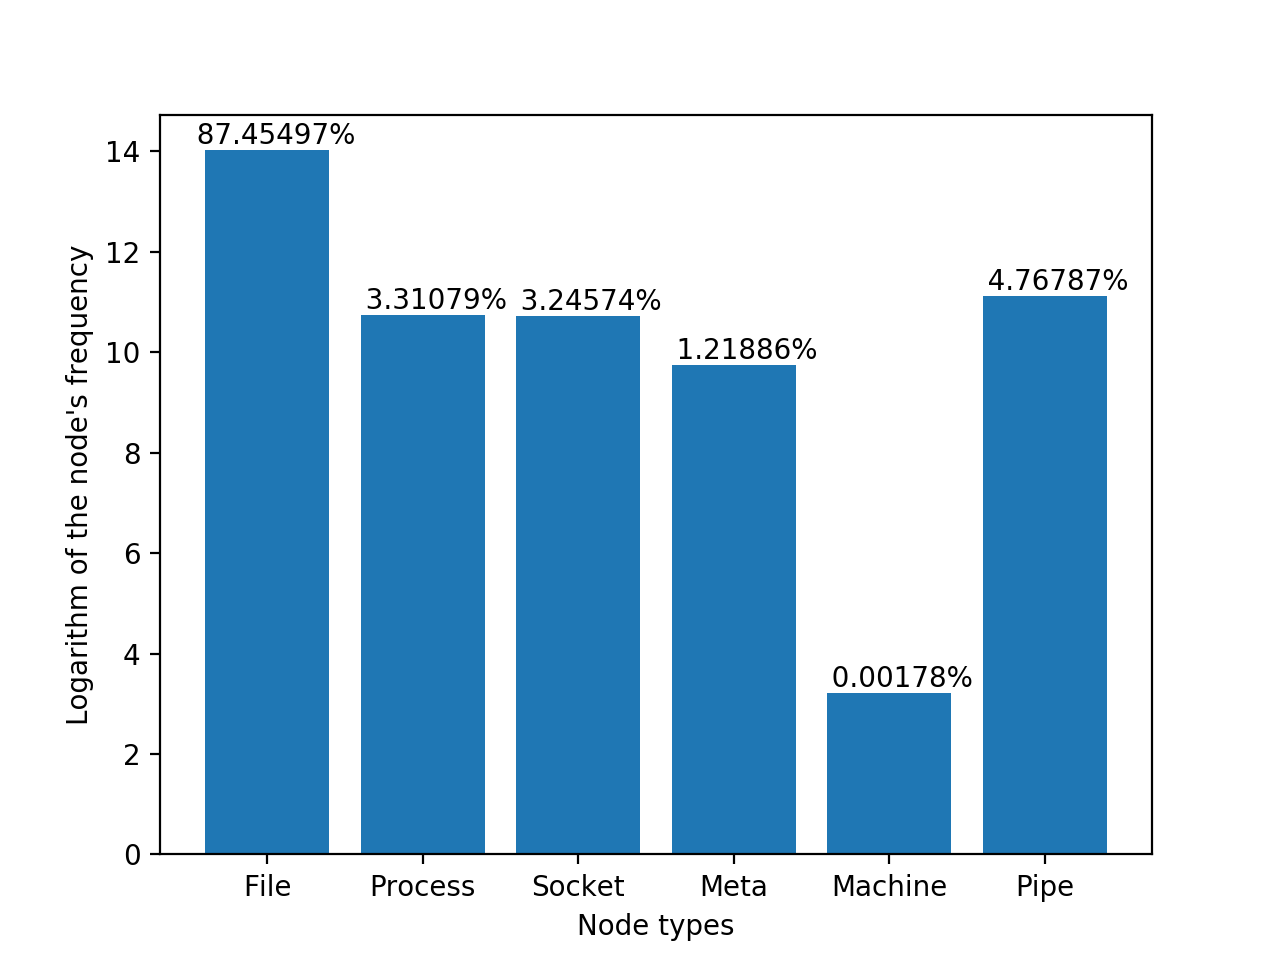
\includegraphics[width=0.7\textwidth]{graphics/node-freq-graph}
		\caption[\textbf{Log-scale node frequency}]{
			Bar chart above showing the log-scale node frequency in a database of $1,402,053$ nodes and $2,090,741$ edges. 
		}
		\label{Figure 2.1.1}
	\end{figure}
	Relationships between nodes are illustrated by different types of edges. Some edges also illustrate how an object (File, Socket, etc.) evolves over time. This is done using the \textit{GLOB\_OBJ\_PREV} edge and helps us to easily visualize the different versions of an object.
	\begin{figure}[H]
		\centering

		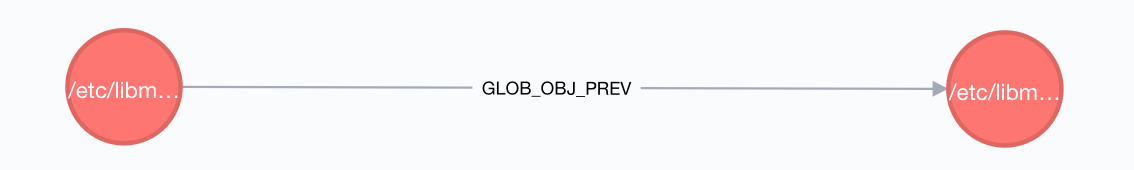
\includegraphics[width=0.7\textwidth]{graphics/GLOB_OBJ_PREV}
		\caption{
			Two versions of the same file connected via a GLOB\_OBJ\_PREV edge.
		}
		\label{Figure 2.1.2}
	\end{figure}
	A number of the edge types also use a \textit{state} field, in order to provide further information regarding the relationship between two nodes. For example, in the case of a \textit{PROC\_OBJ} edge connecting a File to a Process, the \textit{state} field is used to show whether the Process reads/ writes to the File or if the File is the binary the Process is executed from. \textit{PROC\_OBJ} edges also connect Processes to Sockets. Here, the \textit{state} field can take values such as: \textit{Server} (if the Process uses the Socket to accept new connections), \textit{Client} (if the Process uses to Socket to connect to a different Process that acts as a server - which may or may not be on a different machine)  and \textit{RaW} (if the Process also reads and writes through the Socket).
	\begin{figure}[H]
		\centering
		
		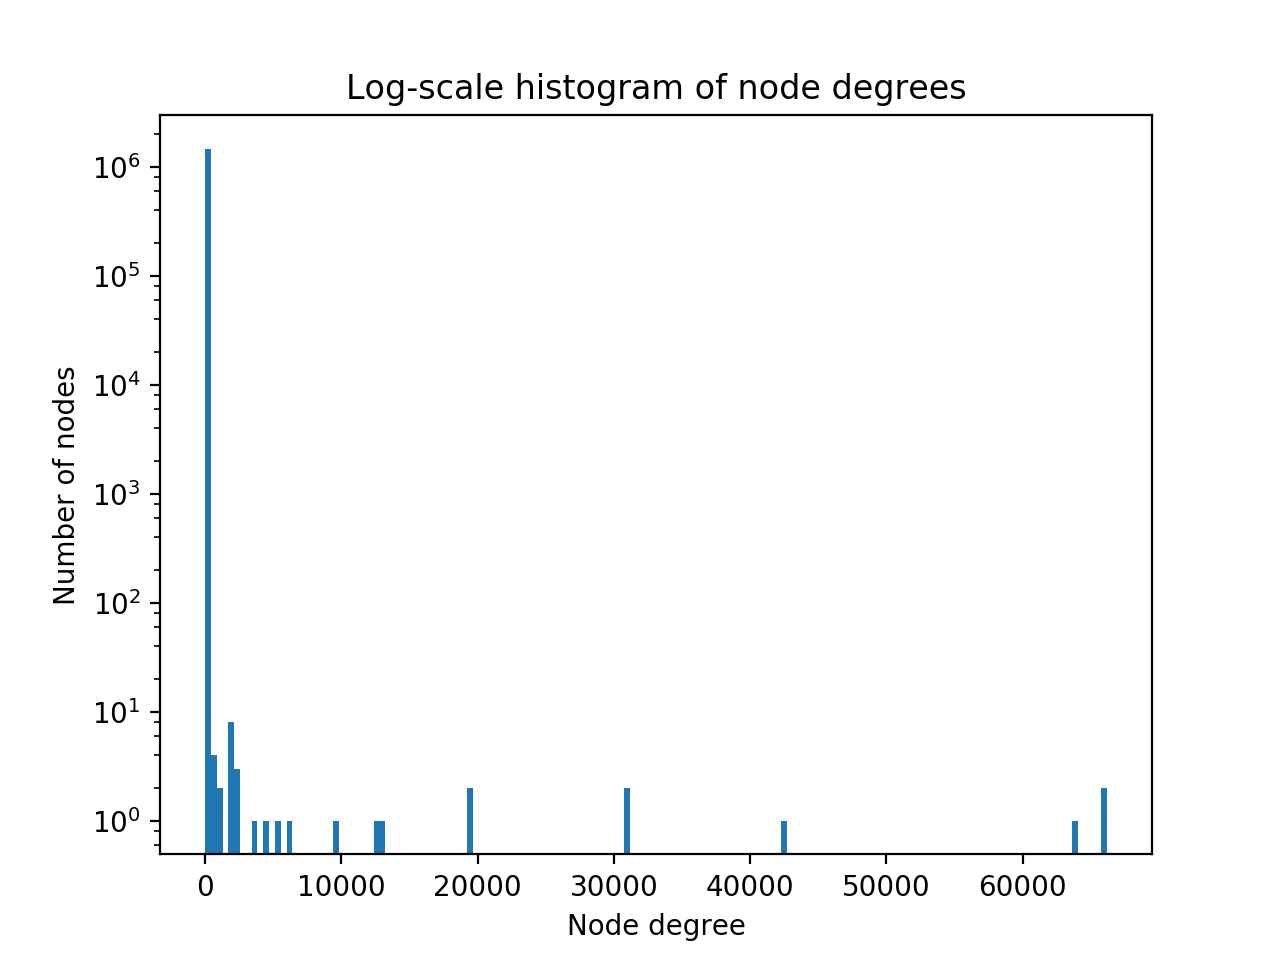
\includegraphics[width=0.7\textwidth]{graphics/node_degree_hist}
		\caption[Log-scale distribution of node degrees]{
			Log-scale histogram showing the distribution of node degrees, using the same graph as the one from Figure \ref{Figure 2.1.1} as source(i.e. $1,402,053$ nodes and $2,090,741$ edges).
		}
		\label{Figure 2.1.3}
	\end{figure}
	 
	 The graphs resulting from tracing are very sparse, with a number of edges almost equal to the number of nodes. This observation is also sustained by the histogram in Figure \ref{Figure 2.1.3}, where we can observe that most of the nodes have degrees between 0 and 10, while there also are a few nodes with a very high degree (up to $60, 000$). Therefore, the degrees of the nodes encountered in the database follow a power-law distribution\cite{Clauset:2009:PDE:1655787.1655789}.
	 
	\subsection{Ground truths} \label{Section: prep/data/ground-truths}
	In order to apply appropriate supervised learning algorithms, I had to build a labelled dataset of nodes from the raw data stored in graph format. This required setting a number of \textit{ground truths} of what a node of interest is. 
	\\ \\
	These ground truths are represented by a set of 6 rules, where I took into consideration a subset of node types: Files, Processes and Sockets. The rules are:
	\begin{enumerate}
		
		\item \textbf{Sockets that connect to an external IP: }Any socket that connects to an IP address other than 127.0.0.1 (localhost) can be considered a possible security breach because it could be used to leak information.
		
		\item \textbf{Files downloaded from the web and then executed: }Any file downloaded from the web can be suspicious, because we can not trust the source. Especially if it is executed, it can pose a real security threat to the system. The graph representation in the Neo4J database can be seen in Figure \ref{Figure 2.3}.
		\begin{figure}[H]
			\centering
			\includegraphics[width=0.7\textwidth]{graphics/downloaded-and-executed}
			\label{Figure 2.3}
			\caption{Graph representation of a file downloaded and then executed}
		\end{figure}
		In the figure above, Process1 writes the File while it is connected to the Socket and then Process2 starts, using File as binary.
		
		\item \textbf{File read from/ written to by a Processes that also opens a Socket to a different machine: }Here are two cases we need to treat separately. If the Process reads from the File, we face a potential leak of the File's contents. If the Process writes to the File, on the other hand, it might be the case that it corrupts its contents. This is a potential threat especially if the File is a sensitive file of the operating system (e.g. any file in /lib/ or /bin/). 
		
		\item \textbf{Processes that open a Socket to a different machine: }As mentioned at point 1, any Socket connecting to an external machine is a potential threat. In the same time, any process that opens a Socket to a different machine can be a source of suspicious behaviour, as well. 
		
		\item \textbf{Processes that runs suspicious commands: }Here, I define the term of \textit{suspicious command} as being one of the following bash commands:
		\begin{itemize}
			\item \textit{sudo} - gives the user running the Process root privilege. An attacker might use this to access OS-sensitive locations (such as /bin or /lib). 
			\item \textit{usermod/ groupmod} - an attacker might make use of these commands to change the running user's privileges and access files that it wouldn't otherwise have access to.
			\item \textit{chmod} - an attacker might use this command to change the access control to a specific File in order to make it accessible from external sources.
			\item \textit{rm -rf} - an ill-intended user might use this command to delete files crucial to the system. 
		\end{itemize}
	
		\item \textbf{Processes that writes to files in suspicious locations: }Here, I define the term of \textit{suspicious location} as being a location that is essential to the running of the system. These locations include:  \textit{/bin, /etc, /lib, /usr/bin, /usr/lib, /boot, /root, /dev, /etc/pwd}.
	\end{enumerate}
	These rules only represent a suitable starting point for the tool implemented here. In practice, though, I would expect my model to be driven by past analyst observations and interactions in the UI. This is a fact I kept in mind when considering various machine learning models, in order to try to create ones that can be updated given analyst input.
	\\ \\
	By setting these ground-truths, this project is also exploring whether the various machine learning algorithms implemented as part of this project can easily learn a number of patterns in the same time.
	\subsection{Data preprocessing} \label{Section: prep/data/feature-vectors}
	The implemented machine learning models only look at 3 of the 6 types of nodes: \textbf{File}, \textbf{Process} and \textbf{Socket} nodes. 
	\\ \\
	In order to achieve this, I had to define a set of features that would construct the \textit{feature vectors} representing each node. Furthermore, for graph-specific models (such as Graph Attention Networks, described in section \ref{Section 2.2.4})  I also built the adjacency matrix of the given graph. 
	\\ \\
	I defined 13 features that would describe each node, in the same time taking into account its 'neighbour'. For a Process, the neighbour is the closest File or Socket connected to it. Here, \textit{'the closest node'} is the node that with the closest timestamp to it. Similarly, for a File or Socket, the neighbour is the closest Process node connected to it.
	
	%%%%%%%%%%%%%%%%%%%%%%%%%%%%
	%%%%%% FEATURES TABLE %%%%%%%%%%
	%%%%%%%%%%%%%%%%%%%%%%%%%%%%
	
	\begin{longtable}{| p{.12\textwidth} || p{.22\textwidth} | p{.22\textwidth} | p{.22\textwidth} | p{.15\textwidth} |}
		\hline
		\multirow{2}{3cm}{\textbf{Feature}} & \multicolumn{3}{c|}{\textbf{Explanation}} & \multirow{2}{2cm}{\textbf{Type}}\\
		& Process & Socket & File &\\
		\hline
		\textit{Node type} & \multicolumn{3}{c|}{The type of node used in this case (i.e. Process, Socket or File)} & \textbf{Categorical} \\
		\hline
		\textit{Neighbour type} & The closest node connected to it. Has to be one of File and Process & 
		\multicolumn{2}{c|}{Will always be Process} & \textbf{Categorical}\\
		\hline
		\textit{Edge type} & \multicolumn{3}{p{.75\textwidth}|}{The type of edge connecting the node to the neighbour. It will always be a $PROC\_OBJ$ edge, but the \textit{state} field can take multiple values, such as:  \textit{READ, WRITE, RaW, BIN, SERVER, CLIENT, NONE}.} & \textbf{Categorical}\\
		\hline
		\textit{Connected} & Whether the Process in question connects to a different machine via a Socket. & Whether the Sockets connects to an IP address other than 127.0.0.1. & Whether the File was downloaded from the web or not. & \textbf{Binary} \\
		\hline
		\textit{Neighbour connected} & \multicolumn{3}{c|}{Whether the neighbour is Connected or not.} & \textbf{Binary} \\ 
		\hline
		\textit{UID status} & Whether the uid is equal to the euid for the Process in question or not. & \multicolumn{2}{p{.50\textwidth}|}{Whether the uid is equal to the euid for the corresponding Process neighbour or not.} & \textbf{Binary} \\
		\hline
		\textit{GID status } & Whether the gid is equal to the egid for the Process in question or not. & \multicolumn{2}{p{.50\textwidth}|}{Whether the gid is equal to the gid for the corresponding Process neighbour or not.} & \textbf{Binary} \\
		\hline
		\textit{Version} & \multicolumn{3}{p{.75\textwidth}|}{The version number of the current node (i.e. how many nodes with the same ID and smaller timestamp are present in the graph.)} & \textbf{Integer} \\
		\hline
		\textit{Suspicious} & Whether the process accesses files in a restricted directory (eg: \textit{/etc/pwd, /usr/bin, /usr/lib, /bin, /lib}), whether the command starting the process contains keywords such as: \textit{sudo, chmod, usermod, groupmod, rm -rf}. & Whether the Process that initiated the Socket has the \textit{Suspicious} flag or not &Whether the file in question has a suspicious name, containing keywords such as: \textit{attack, worm, trojan, virus, etc.} & \textbf{Binary} \\
		\hline
		\textit{External} & Whether it connects to a different machine via a Socket. & Whether the Socket is to an IP address other than 127.0.0.1. & Whether the File contents are transmitted via a Socket to a different machine. & \textbf{Binary} \\
		\hline
		\textit{Degree} & \multicolumn{3}{c|}{The degree of the node in question.} & \textbf{Integer} \\
		\hline
		\textit{Neighbour degree} & \multicolumn{3}{c|}{The degree of the Neighbour} & \textbf{Integer} \\
		\hline
		\textit{Neighbour distance} & \multicolumn{3}{p{.75\textwidth}|}{
			\makecell{
			\begin{math}
				=
				 \begin{cases} 
					0.0 & \text{if } \Delta t = 0\\
					\log \Delta t & \text{otherwise} 
				\end{cases} 
			\end{math}
			\\
			where $\Delta t = abs(node.timestamp - neighbour.timestamp)$ 
		} } & \textbf{Real} \\
	\hline
	\caption[Features table]{\centering Table listing and explaining the meaning of the features that are extracted for every node.}
	\label{Table: prep/features}
	\end{longtable}


	\section{Machine learning models} \label{Section 2.2}
	This section describes the underlying theory of the machine learning models explored as part of this project and how they can be applied to the data I am working on.

	\subsection{Supervised learning using neural networks} \label{Section 2.2.2}
	Given a training sequence $\mathbf{s} = [(\mathbf{x_1}, y_1), (\mathbf{x_2}, y_2) \dots (\mathbf{x_m}, y_m)]$, a neural network learns a hypothesis $h: \mathbb{R}^n \rightarrow \mathcal{C}$ that maps an input feature vector $\mathbf{x}$ to its corresponding label $y$. 
	\\ \\
	The hypothesis is set as $h(\mathbf{x}) = f(\mathbf{x}; \mathbf{w}, \mathbf{b})$, where $f$ is a function dependent on the neural network architecture and $\mathbf{w}$ and $\mathbf{b}$ are the weights and biases, respectively. 
	\\ \\
	A \textbf{loss function} is usually defined to measure some notion of the neural network's error when estimating $y$ from $\mathbf{x}$, given $\mathbf{w}$ and $\mathbf{b}$. The training step involves an optimisation algorithm which aims at finding $\mathbf{w}$ and $\mathbf{b}$ such that the loss function is minimized. 
	
 	\subsubsection{Multilayer perceptron}  \label{Section 2.2.2.2}
	Neural network architectures consist of multiple interconnected artificial neurons in order to infer complex functions. The mutilayer perceptron (MLP) represents a class of feedforward artificial neural networks (ANN) where the neurons are arranged in three or more layers (as shown in Figure \ref{Fig: prep/ml/mlp/mlp}). MLPs are \textbf{fully connected}; that is each neuron in one layer connects to every neuron in the following layer with a certain weight $w_{i, j}$

	\begin{figure}[H]
		\centering
		\includegraphics[width=0.7\textwidth]{graphics/nns/multilayer}
		\caption[Multilayer perceptron]{
			Figure showing a 2-layer neural network.
		}
		\label{Fig: prep/ml/mlp/mlp}	
	\end{figure}	

	 Each layer of the MLP consists of a number of neurons(Figure \ref{Fig: prep/ml/mlp/neuron}). For an input vector $\mathbf{x}\in\mathbb{R}^d$, a weight vector $\mathbf{w}\in\mathbb{R}^d$, and a biast $b$, a neuron computes the output $y = \sigma(b + \sum_{i=1}^{d} w_i x_i)$, where $\sigma$ is an \textit{activation function}.
	
	\begin{figure}[H]
		\centering
		
		\includegraphics[width=0.7\textwidth]{graphics/nns/single_neuron}
		\caption[\textbf{Artificial neuron}]{
			Figure showing a single artificial neuron. 
		}
		\label{Fig: prep/ml/mlp/neuron}
	\end{figure}
	\subsubsection*{Activation functions}
	The main purpose of using an activation function $\sigma$ is to map the output of the linear combination of input features onto a desired (finite) range. Moreover, choosing the appropriate activation function can speed up the training process and even help us avoid the overfitting problem. Some frequently encountered activations functions are:
	\begin{enumerate}
		\item the \textbf{linear function}
		\begin{equation}
		\sigma(x) = cx 
		\end{equation}
		where $c \in \mathbb{R}$ is a constant. 
		
		\item the \textbf{sigmoid function}
		\begin{equation}
		\sigma(x) = \frac{1}{1+e^{-x}}
		\end{equation}
		
		\item the \textbf{tanh function}
		\begin{equation}
		\sigma(x) = \tanh(x) = \frac{2}{1+e^{-2x}} - 1
		\end{equation}
		Essentially, the $\tanh$ function is a scaled sigmoid function. It can be re-written as: $\tanh(x) = 2 \times \text{sigmoid}(2x) - 1$ 
		
		\item the \textbf{rectified linear unit (ReLU) function}
		\begin{equation}
		\sigma(x) = 
		\begin{cases}
		0 & \text{if } x < 0 \\
		x & \text{if } x \geq 0
		\end{cases}
		\end{equation}
		
		\item the \textbf{leaky rectified linear unit (LReLU) function}
		\begin{equation}
		\sigma(x) = 
		\begin{cases}
		0.001x & \text{if } x < 0 \\
		x & \text{if } x \geq 0
		\end{cases}
		\end{equation}
	\end{enumerate} 
	In the past, the $\tanh$ used to be the activation function of choice in neural networks, but recent works\cite{nonlinearities} have shown that rectified nonlinearities (such as ReLU or LReLU) considerably improve the performance of the model. Figure \ref{Fig: prep/ml/mlp/activations} shows the graphs of three of the activation functions above ($\tanh$, ReLU and LReLU) and their derivatives.
	\begin{figure}[H]
		\centering
		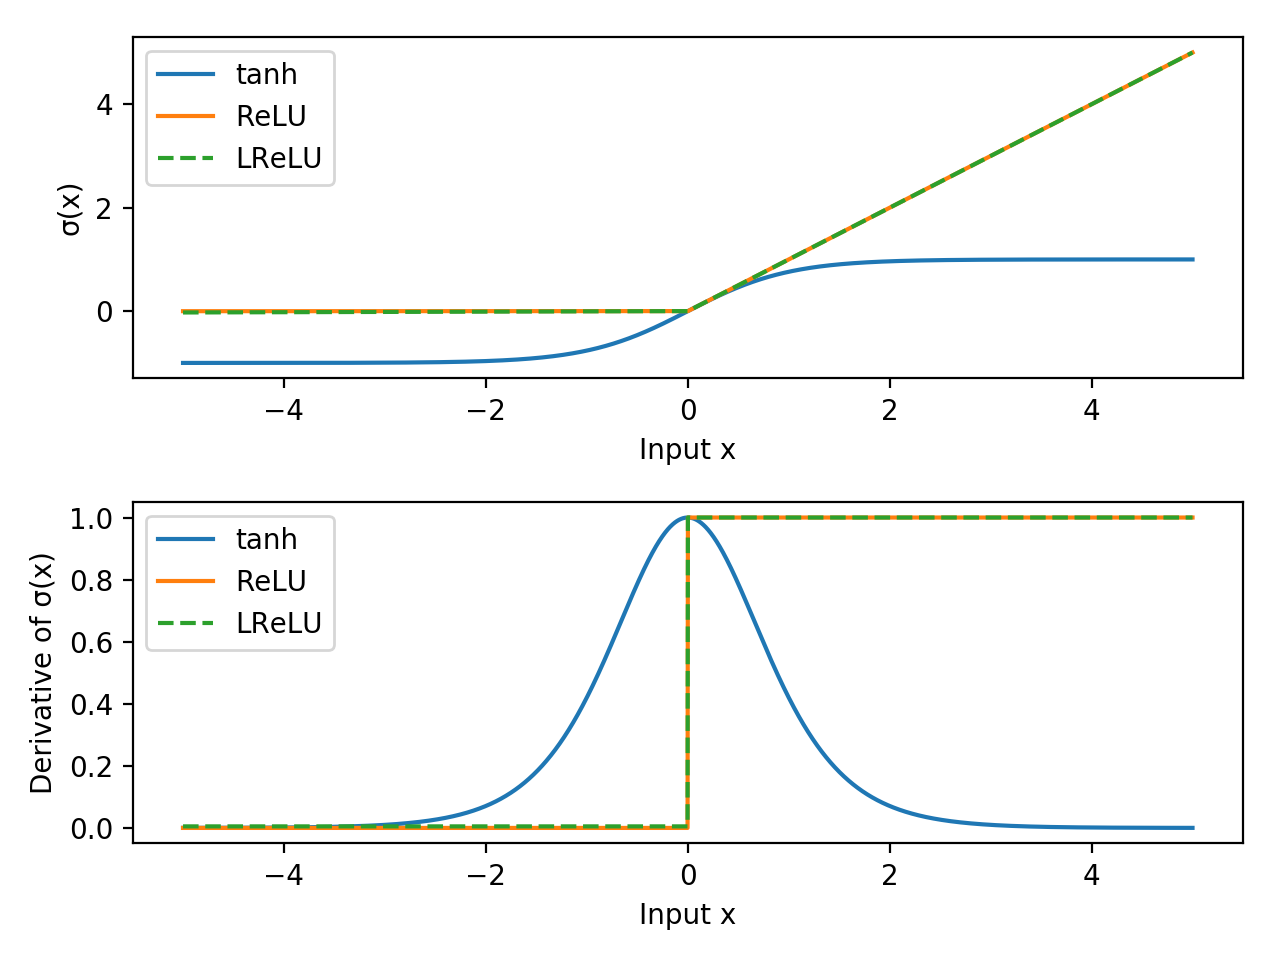
\includegraphics[width=0.7\textwidth]{graphics/nns/activations}
		
		\caption[Activation functions]{The $\tanh$, ReLU and LReLU functions and their derivatives}
		\label{Fig: prep/ml/mlp/activations}
	\end{figure}
	In general, neural networks are optimised using gradient-based algorithms. Therefore, activation functions with steeper gradients (such as ReLU and LReLU) tend to make the algorithm to converge faster.
	
	\subsubsection*{Using MLPs for classification}
	In this project, I intend to classify nodes as being in one of two classes: \textit{SHOW} and \textit{HIDE}, based on the feature vectors described in Section \ref{Section: prep/data/feature-vectors}. Therefore, we are interested in seeing how an MLP can be used to solve classification problems. As shown by Cybenko's theorem\cite{sigmoidal}, MLPs are universal function approximators, so that they can be used to create mathematical models by regression analysis. Considering the fact that classification is a particular case of regression where the response variable is categorical, we can infer that MLPs make good classifier algorithms. 
	\\ \\
	Suppose the MLP has to learn to classify a feature vector $\mathbf{x} \in \mathbb{R}^d$ into a class $C_t$ from $\mathcal{C} = \{C_1\dots C_k\}$. In this case, we want the $t^{th}$ output neuron (i.e. $o_t$) to indicate this. A popular choice for this task is the \textbf{softmax function}, which transforms any k-dimensional vector $\mathbf{o}$ to the probability distribution:
	\begin{equation}
		\centering
		\text{softmax}_i(\mathbf{o})_i = \frac{e^{o_i}}{\sum_{j=1}^{k}e^{o_j}}
	\end{equation}
	where: $\mathbf{o}^T = [o_1\dots o_k]$ is the vector of the output neurons. Thus, the probability of the input vector $\mathbf{x}$ being in class $C_t$ is given by:
	\begin{equation}
		\centering
		\begin{split}
			\mathbb{P}(y = C_t | \mathbf{x}) & = \text{softmax}_i(\mathbf{o})_t \\
			& = \frac{e^{o_t}}{\sum_{j=1}^{k}e^{o_j}}
		\end{split}
		\label{Eq: prep/ml/mlp/softmax}
	\end{equation} 
	
	If we consider the hidden layer from Figure \ref{Fig: prep/ml/mlp/mlp} to use the ReLU activation function, we can re-write the equation \ref{Eq: prep/ml/mlp/softmax} in vector format as follows: 
	\begin{equation}
		\centering
		\mathbb{P}(y=C_t | \mathbf{x}) = \frac
		{
			\exp (\mathbf{W_2}\text{ReLU}(\mathbf{W_1 x} + \mathbf{b_1}) + \mathbf{b_2})_t
		}
		{
			{\sum_{j=1}^{k}\exp (\mathbf{W_2}\text{ReLU}(\mathbf{W_1 x} + \mathbf{b_1}) + \mathbf{b_2})_j}
		} 
	\end{equation}
	
	where $\mathbf{x}$ is the input feature vector.
	
	\subsubsection*{Training the MLP}
	Using a training sequence $\mathbf{s}$, the parameters of the MLP have to be optimised in order to be able to have a performant classifier. One of the most frequently used optimisation techniques is \textbf{gradient descent}, which updates the parameters iteratively, by moving in the direction of the gradient of a loss function. In a complex system, the gradient is calculated using \textbf{backpropagation}. This algorithm is described in detail in Appendix \ref{appendix-MLP-opt}. 
	
	\subsection{Convolutional Neural Networks} 
	Classically, Convolutional Neural Networks(CNNs) are used in tasks such as computer vision or natural language processing. One-dimensional CNNs, though, have proven to be effective for non-spatial data, as well, by identifying relations between the features from the input feature vectors. For this reason, I considered this as a potential model in my project. 
	\\ \\
	CNN make use of \textbf{convolutional layers} in order to identify relations between features in a subarea of the feature vector. 	Following these convolutional layer(s), a CNN normally has a one or more fully connected layers that process the outputs and return either a probability distribution (for classification) or a single value (in the case of regression).  
	
	\subsubsection*{Convolutional layer}
	The main purpose of the convolutional layer is to extract relationships between the features from an input vector. It uses a fix-sized kernel $\mathbf{w} \in \mathbb{R}^k$, that slides over the input vector $\mathbf{x}\in\mathbb{R}^d$ and computes a linear transformation for every patch of size $k$. The output of the convolutional layer is a new vector $\mathbf{y}\in\mathbb{R}^n$, where $n=d - k + 1$. The values of each element in the output vector is given by the equation:
	\begin{equation}
		y_i = \mathbf{w}^T\mathbf{x}_{i:i+k-1}
	\end{equation}
	where $\mathbf{x}_{a:b}$ represents the sub-vector containing all elements $x_i. \forall a\leq i \geq b$. Figure \ref{Fig: prep/ml/cnn/convoLayer} shows the step-by-step construction of the output vector.
	\begin{figure}[H]
		\centering
		\begin{subfigure}[b]{0.3\linewidth}
			\includegraphics[width=\linewidth]{graphics/nns/conv/1}
			\vspace*{1cm}
		\end{subfigure}
		\begin{subfigure}[b]{0.3\linewidth}
			\includegraphics[width=\linewidth]{graphics/nns/conv/2}
			\vspace*{1cm}
		\end{subfigure}
		\begin{subfigure}[b]{0.3\linewidth}
			\includegraphics[width=\linewidth]{graphics/nns/conv/3}
			\vspace*{1cm}
		\end{subfigure}
		\begin{subfigure}[b]{0.3\linewidth}
			\includegraphics[width=\linewidth]{graphics/nns/conv/4}
		\end{subfigure}
		\begin{subfigure}[b]{0.3\linewidth}
			\includegraphics[width=\linewidth]{graphics/nns/conv/5}
		\end{subfigure}
		\begin{subfigure}[b]{0.3\linewidth}
			\includegraphics[width=\linewidth]{graphics/nns/conv/6}
		\end{subfigure}
		\caption[1D Convolution]{Step-by-step example of 1D convolution with a $1\times3$ kernel}
		\label{Fig: prep/ml/cnn/convoLayer}
	\end{figure}
	In order to add further nonlinearity and prevent the overfitting of the model, one may also use an activation function $\sigma$ when computing the final outputs of the layer. Furthermore, in order to manipulate the length of the output vector, we can also use \textbf{zero-padding}, which simply pads the input vector with zeros, such that the output preserves its length.
	\\ \\
	\textbf{Dilated convolution}(Figure \ref{Fig: prep/ml/cnn/dilated}) is a technique that increases the receptive (global) view of the network exponentially and has proven extremely effective in tasks such as context and text-to-speech resolution. In this case, the filter (kernel) is applied over a larger area than its length by skipping input values with a certain step, called \textit{dilation field}. Exponentially increasing the dilation rate results in an exponential field growth in depth\cite{DBLP:journals/corr/YuK15}.  
	\\ \\
	Recent work has shown that dilated convolution is a simple by effective idea when it comes to detection of fine-grained details by processing inputs in higher resolutions. For this reason, I have considered applying this approach to the problem at hand.
	
	\begin{figure}[H]
		\centering
		\includegraphics[width=.8\textwidth]{graphics/nns/conv/dilated}
		\caption[Dilated convolution]{Dilated convolution schema reproduced from \textit{van den Oord et al.} \citep{DBLP:journals/corr/OordDZSVGKSK16}}
		\label{Fig: prep/ml/cnn/dilated}
	\end{figure}

	\subsection{Graph Attention Network}	
	This section describes Graph Attention Networks (GATs), state-of-the-art neural network architectures that operate on graph-structured data (as described by \cite{2017arXiv171010903V}). It is based on the attentional mechanisms that have proven to be extremely effective in tasks such as Neural Machine Translation (NMT)\cite{DBLP:journals/corr/LuongPM15, DBLP:journals/corr/VaswaniSPUJGKP17}. One of the benefits of these mechanisms is the fact that they allow for dealing with variable sized inputs, focusing on the most relevant parts of the input to make decisions. 
	\\ \\
	Unlike the other models discussed in this section, GATs take full advantage of the relational structure of the graph, by not treating the nodes as being isolated, but instead also looks at the neighbourhood of every node (i.e. the nodes being at mostly one hop distance from the one we want to classify). For this reason I considered this architecture as a potentially interesting model for the classification problem I am trying to solve.
	\\ \\ 
	By stacking layers in which nodes are able to attend over their neighbourhood's features, GATs enable specifying different weights to different nodes in a neighbourhood, without requiring any kind of costly matrix operations or depending on knowing the graph structure upfront. 
	\\ \\
	All GAT architectures include at least one \textbf{graph attentional layer}. The layer takes as input a set of node features, $\mathbf{s} = \{\mathbf{h}_1, \mathbf{h}_2, \dots , \mathbf{h}_N \}$, $\mathbf{h}_i \in \mathbb{R}^F$, where $N$ is the number of nodes and $F$ is the number of features of each node. It outputs a new set of node features( of potentially different cardinality $F'$) $\mathbf{s'} = \{ \mathbf{h'}_1, \mathbf{h'}_2, \dots , \mathbf{h'}_N \}$. In order to achieve this, it performs self-attention on the nodes - using a shared attentional mechanism $a:\mathbb{R}^{F'}\times\mathbb{R}^{F'}\rightarrow\mathbb{R}$ that computes the attention coefficients $e_{i,j}$:
	\begin{equation}
		e_{i,j} = a(\mathbf{W}\mathbf{h}_i, \mathbf{W}\mathbf{h}_j)		
	\end{equation} 
	where $\mathbf{W}$ is a weight matrix that is used to apply linear transformations to every node. Each attention coefficient $e_{i,j}$ indicates the importance of $j$'s features to node $i$. In order to take the graph structure into consideration, we compute $e_{i,j}$ only for the nodes $j \in \mathcal{N}_i$, where $\mathcal{N}_i$ is the neighbourhood of node $i$ in the graph. We want our coefficients to be easily comparable across different nodes, we normalize attention coefficients:
	\begin{equation}
		\alpha_{i,j} = \text{softmax}_j(e_{i,j}) = \frac{\exp(e_{i,j})}{\sum_{k\in \mathcal{N}_i} \exp(e_{i,k})}
	\end{equation}
	Once obtained, the normalized attention coefficients can be used to compute the new set of node features, $\mathbf{s} = \{ \mathbf{h'}_1, \mathbf{h'}_2, \dots , \mathbf{h'}_N  \}$. Each new feature vector $\mathbf{h'}_i$ is computed using the formula:
	\begin{equation}
		\mathbf{h'}_i = \sigma \Bigg( \sum_{j \in \mathcal{N}_i} \alpha_{i,j} \mathbf{W} \mathbf{h}_j \Bigg) 
	\end{equation}
	where $\alpha$ is a nonlinear activation function. 
	\subsection{Non-parametric techniques}	\label{Section 2.2.5}
	So far, I discussed various parametric machine learning techniques I considered appropriate for the problem I am trying to solve. These models, though, treat supervised learning under the assumption that the forms of the underlying density functions were known, even though they rarely fit the densities actually encountered in practice. 
	\\ \\
	In this section, I examine how the probability density functions of the two classes (i.e. \textit{SHOW} and \textit{HIDE}) can be estimated from a sequence of labelled training data, using the non-parametric model called Probabilistic Neural Networks (PNNs). Firstly, they rely on the fact that the probability $P$ that a real vector $\mathbf{x}$ falls in a region $\mathfrak{R}$ is given by:
	\begin{equation}
		\centering
		P = \int_{\mathfrak{R}} p(\mathbf{x'}) d\mathbf{x'}
	\end{equation}
	Thus, $P$ is a smoothed version of the density function $p(\mathbf{x})$. Suppose that $m$ samples $\mathbf{x}_1,\dots ,\mathbf{x}_n$ are drawn independently and identically distributed (i.i.d.) accordingly to the probability law $p(\mathbf{x})$. The probability that $k$ of these $m$ fall in $\mathfrak{R}$ is given by the binomial law:
	\begin{equation}
		P_k = {n\choose k} P^k (1-P)^{n-k}
	\end{equation}
	and the expected value for $k$ is: $\mathbb{E}(k) = nP$. Moreover, this distribution for $k$ peaks about the mean so we expect that $\frac{k}{n}$ will be a very good estimate for the probability $P$. This is especially accurate for a very large $m$. 
	\\ \\
	Assuming $p(\mathbf{x})$ is continuous and the region $\mathfrak{R}$ is so small that $p$ does not vary appreciably with it, we can write:
	\begin{equation}
		 \begin{split}
p(\mathbf{x}) &\approx \frac{P}{V} \\
&\approx \frac{k / n}{V}
\end{split}	
	\label{Eq-np 1}
	\end{equation}
	where $\mathbf{x}$ is a point in $\mathfrak{R}$ and $V$ is the volume of the region $\mathfrak{R}$.
	\\ \\
	The equation \ref{Eq-np 1} behaves poorly when the volume $V$ approaches 0. Therefore, we want to estimate the density of $\mathbf{x}$ instead. We can do it iteratively by from a sequence of regions $\mathfrak{R}_1, \mathfrak{R}_2, \dots$, each containing $\mathbf{x}$ and every region $\mathfrak{R}_n$ being used with $n$ samples. Let $V_n$ be the volume of $\mathfrak{R}_n$, $k_n$ be the number of samples falling in $\mathfrak{R}_n$ and $p_n(\mathbf{x})$ the $n^\text{th}$ estimate for $p(\mathbf{x})$:
	\begin{equation}
		p_n(\mathbf{x}) = \frac{k_n/n}{V_n}
		\label{Eq-np 2}
	\end{equation}
	
	\subsubsection{Parzen windows}
	This section describes the Parzen-window approach to estimating densities. It assumes that the region $\mathfrak{R}_n$ is a d-dimensional hypercube, where $h_n$ is the length of an edge. Then, we can estimate the volume $V_n = h_n^d$. Let $\varphi$ be the window function:
	\begin{equation}
		\varphi(\mathbf{u}) = \begin{cases}
											 1 & |u_j| \leq \frac{1}{2}, \forall j \in \{1\dots d\} \\
											 0 & \text{otherwise}
									   	\end{cases}
	\end{equation}
	Thus, $\varphi(\mathbf{u})$ defines a unit hypercube centered at origin. It follows that $\varphi(\frac{\mathbf{x} - \mathbf{x}_i}{h_n})$ is equal to $1$ if $\mathbf{x}_i$ falls in hypercube of volume $V_n$, centered at $\mathbf{x}$ and $0$ otherwise. Therefore, the number of samples in this hypercube $k_n$ is given by:
	\begin{equation}
		k_n = \sum_{i=1}^{n} \varphi \bigg(\frac{\mathbf{x} - \mathbf{x}_i}{h_n}\bigg)
	\end{equation}
	By fitting this into equation \ref{Eq-np 2}, we can obtain the $n^{\text{th}}$ estimate of the probability distribution function $p_n(\mathbf{x})$: 
	\begin{equation}
		p_n(\mathbf{x}) = \frac{1}{n} \sum_{i=1}^{n} \frac{1}{V_n} \varphi \bigg( \frac{\mathbf{x} - \mathbf{x}_i}{h_n} \bigg)
		\label{Eq-np 3}
 	\end{equation} 
 	In the general case, we want to allow more general window functions rather than limiting ourselves to a hypercube unit function. In such a case, the equation \ref{Eq-np 3} expresses our estimate of $p(\mathbf{x})$ as an average of functions of $\mathbf{x}$ and the samples $\mathbf{x}_i$. In essence, the window function is being used for \textit{interpolation} - each sample contributing to the estimate in accordance to the distance from $\mathbf{x}$.
 	
 	\subsubsection{Probabilistic Neural Networks}
 	Probabilistic Neural Networks (PNNs) are classifiers based on Parzen windows. Suppose we want to classify n-dimensional vectors $\mathbf{x} \in \mathbb{R}^n$ into one of $k$ classes in $\mathcal{C}=\{C_1\dots C_k\}$. Based on a training sequence $\mathbf{s} = \{ (\mathbf{x}_1, C), (\mathbf{x}_2, C), \dots ,(\mathbf{x}_m, C)\}$ we estimate the probability density functions $p_i(\mathbf{x}). \forall i \in \{1,2,\dots,k \}$ for every class in $\mathcal{C}$. 

  	\begin{figure}[H]
 		\centering
 		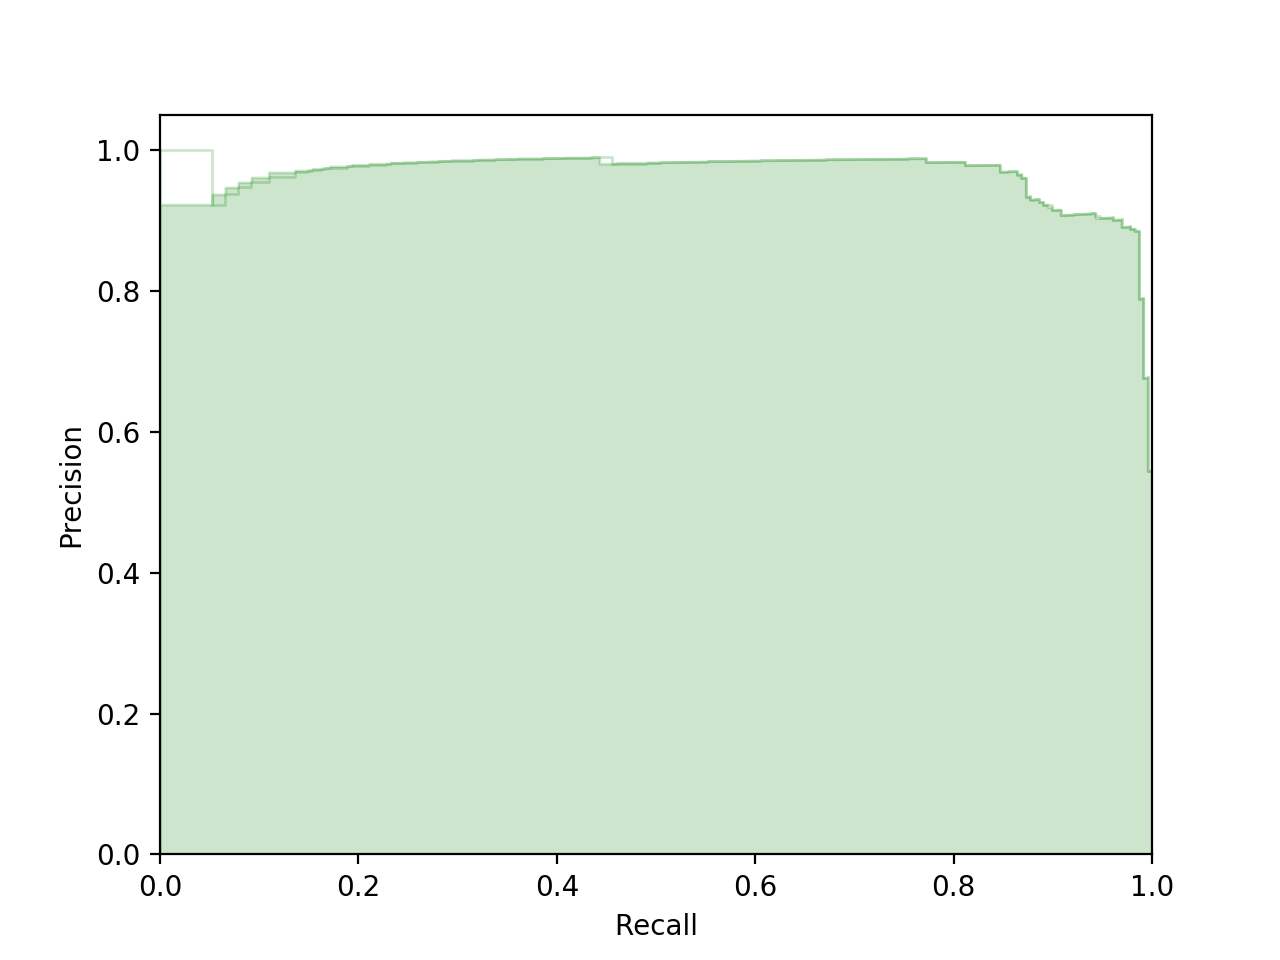
\includegraphics[width=\textwidth]{graphics/nns/pnn}
 		\caption{PNN architecture}
 		\label{Fig 2.8}
 	\end{figure}
	 
	 Figure \ref{Fig 2.8} shows a general-purpose PNN architecture that can be used for classification. It consists of $n$ input units, $m$ pattern units and $k$ output units. Each pattern unit forms the inner product of its weight vector $\mathbf{w}$ and the normalized pattern vector $\mathbf{x}$ and outputs $\exp(\frac{\mathbf{w}^T\mathbf{x} - 1}{\sigma^2})$. Each category unit sums up the outputs of the pattern units connected to it. This insures that the activity in each of the category units represents the Parzen-window density estimate using a circular symmetric Gaussian window of covariance $\sigma^2\mathbf{I}$, where $\mathbf{I}$ is the $n\times n$ identity matrix. $\sigma$ is a parameter set by the user and is equal to $\sqrt{2}$ times the width of the effective Gaussian window
     \\ \\ 
	 The weights of the $p^\text{th}$ pattern unit are set as $\mathbf{w}_p = \mathbf{x}_p$, $\forall p \in \{ 1,2,\dots ,m \}$, where $\mathbf{x}_p$ is the normalised $p^\text{th}$ pattern from the training set. In order to classify the a new normalized pattern $\mathbf{x}$ we first have to propagate the it through the network. Then, the resulting class will be $C_t$, where:
	 \begin{equation}
		 t = \argmax_i c_i(\mathbf{x}). \forall i \in \{1,\dots k\}
	 \end{equation}
	 and $c_i(\mathbf{x})$ is the output of the $i^\text{th}$ category unit.
	\section{API architecture} \label{Section 2.3}
	Once I decided how to pre-process the raw graph data and researched different applicable machine learning models, I looked into solutions to facilitate interaction between the CADETS user interface and the classifiers. It is desirable for the filtering tool and the UI to be decoupled, in order to allow independent evolution of both parties without affecting the other. For this reason, I decided to use a \textit{\textbf{Representational State Transfer (REST) API}}, taking advantage of the HTTP protocol to facilitate communications with the user interface.
	\\ \\
	Unlike other similar protocols such as SOAP or RPC, REST APIs are not constrained to a single communications format and are do not impose any specific parameters order, therefore providing flexibility. REST APIs are stateless, allowing each call to be made independently, containing solely the data necessary to complete itself successfully. Moreover, the different layers involved in a REST APIs' architecture make it highly modular and scalable. 
	\\ \\
	Being stateless, a REST API might increase the per-request overhead significantly by having to handle loads of incoming and outbound calls. Therefore, it is essential that it is designed to encourage the caching of intermediate results.
	
	\section{Requirements analysis} \label{Section 2.4}
	Having reviewed the structure of the raw graph data, the background theory of the machine learning models and the structure that will facilitate interaction with the CADETS user interface, the requirements of the project overall were closely examined. The end goal of this project is to have an independent and modular tool that is able to connect to the CADETS UI and efficiently classify the nodes from a given graph. A breakdown of the project requirements can be visualized in Table \ref{Table 2.2}.
	\begin{longtable}{|p{.51\textwidth}|p{.13\textwidth} p{.13\textwidth} p{.13\textwidth}|}
		\textbf{Requirements} & \textbf{Priority} & \textbf{Risk} & \textbf{Difficulty} \\
		\hline
		Implementation of baseline model & High & Low & Low \\
		MLP Implementation & High & Medium & Medium \\
		Implementation of CNN & Medium & High & Medium \\
		GAT Implementation & High & High & High \\
		PNN Implementation & Medium & Medium & High \\
		Implementation of the server infrastructure & High & Medium & Medium \\
		Server-side caching implementation for previous results & Medium & Low & Low \\
		Comparative evaluation of the implemented machine learning models & High & Medium & High \\
		\hline
		\caption[Requirements overview]{\centering Overview of the high-level requirements, their priorities, risks and difficulties.}
		\label{Table 2.2}
	\end{longtable}
	\section{Choice of tools} \label{Section 2.5}
	This section describes the tools choices that I made in order to meet the requirements described in Section \ref{Section 2.4}. 
	\subsection{Programming languages} \label{Section 2.5.1}
	Early in the planning stage I decided to use Python 3.6.4\footnote{\textbf{\url{https://www.python.org/downloads/release/python-364/}}} as the main programming language. It is extremely popular in both research and industry deep learning communities, providing a large variety of libraries that can be utilised to this end. 
	\\ \\
	Besides Python, I also used the Cypher Data Manipulation Language (DML) in order to interact to the original graph data stored in Neo4J.  
	
	\subsection{Libraries} \label{Section 2.5.2}
	Apart from the Python built-in libraries, I also used the third-party libraries described in Table \ref{Table 2.3}. 
	\begin{longtable}{|p{.15\textwidth} p{.10\textwidth} p{.4\textwidth} p{.25\textwidth}|}
		\textbf{Library} & \textbf{Version} & \textbf{Purpose} & \textbf{Licence}\\
		\hline
		keras & 2.1.5 & Building and running the neural networks. & MIT Licence \\
		numpy & 1.14.2 & Efficient mathematical operations on vectors and matrices. High precision floating-point calculations. & NumPy Licence\\
		scipy & 1.0.0 & Processing frames and evaluating the machine learning models. & SciPy Licence\\
		pandas & 0.22.0 & Working with tabular data-structures & BSD 3-Clause Licence\\
		flask & 0.12 & Handling the HTTP requests in the REST API layer. & BSD 3-Clause Licence\\
		matplotlib & 2.0.0 & Plotting graphs. & PSF Licence \\
		neo4j-driver & 1.5.3 & Querying the Neo4J database. & Apache 2.0 Licence\\
		pymongo & 3.6.1 & Handling the server-side caching of classification results. & Apache 2.0 Licence\\
		\hline
		\caption[Libaries table]{\centering Table showing the third-party libraries used  as part of this project}
		\label{Table 2.3}
	\end{longtable} 
	The library of key importance to the project is \textbf{Keras}, a high-level neural networks API using Tensorflow\footnote{\textbf{\url{https://www.tensorflow.org/}}} as backend. It is a modular and easily extensible library that fits the iterative software development methodology adopted in this project.
	\subsection{Development and testing environment}
	Development work was entirely done on my personal machine -- a 15" Macbook Pro, running MacOS High Sierra (version 10.13.2). The IDE I chose for this project was \textbf{PyCharm}\footnote{\textbf{\url{https://www.jetbrains.com/pycharm/}}}, due to its high flexibility and support for version control and testing.
	\\ \\
	For a project at this scale, version control is crucial. In order to organize my codebase accordingly, I used the \textbf{git} version control environment and synchronized it remotely with the free online hosting service \textit{GitHub}\footnote{\textbf{\url{https://github.com}}}. GitHub was also used as the main backup strategy for this project.
	\\ \\
	A separate GitHub repository was used to maintain the \LaTeX \space code for this dissertation. 
	
	\section{Starting point} \label{Section 2.6}
	At the start of this project, I had intermediate knowledge of Python, having used it in the Part 1B group project and a number of other small personal projects. However, having had no previous experience with Keras, I had to become acquainted with the API and to learn how to use it to configure neural networks.   
	\\ \\
	In terms of theoretical background, the Artificial Intelligence I course provided sufficient initial knowledge to understand the high-level behaviour of MLPs. Additional research was required to understand the CNNs, GATs and non-parametric techniques implemented. The full list of Tripos courses that were applicable to the project can be seen in Table \ref{Table 2.4}.
	
	\begin{longtable}{|p{.40\textwidth} | p{.50\textwidth}|}
		\textbf{Course} & \textbf{Applicability} \\ 
		\hline
		Artificial Intelligence I & Basic machine learning and neural networks \\
		Databases & Interacting with the Neo4J database \\
		Concurrent \& Distributed Systems & REST API setup \\ 
		Networking & Handling HTTP requests \\
		Operating Systems & High-level understanding of UNIX-based operating systems\\
		Security I & Basic notions of UNIX security setup \\
		\hline
		\caption[Computer Science Tripos courses and their applicability to this project.]{\centering Computer Science Tripos courses and their applicability to this project.}
		\label{Table 2.4}
	\end{longtable}
	
	\section{Software engineering techniques} \label{Section 2.7}
	For the purpose of this project, I decided to use the \textbf{Iterative and Incremental Development Model}. I divided the overall project into three separate modules: 
	\begin{enumerate}
		\item An \textit{interface that communicates with the Neo4J database} in order to extract the features vectors that are used by the machine learning models.
		\item The actual \textit{machine learning models}. 	An initial implementation was developed for each model, which was iteratively refined in order to improve its performance.  
		\item The \textit{server interface} that would handle requests from the CADETS client.
	\end{enumerate}

	\section{Summary} \label{Section 2.8}
	In this chapter I discussed the data the machine learning models work on and how it is preprocessed, the background theory that had to be understood and the software engineering decision that were made before the work could begin. I have presented a condensed theory of the models that were implemented as part of this project. I have also described how the machine learning models will interact with the external sources (i.e. the Neo4J database and the CADETS UI).
	\\ \\
	The next chapter will provide a detailed breakdown of the implementation, showing how the aims described here were accomplished. 
	
\end{document}